\documentclass[a4paper,12pt]{scrartcl}
\usepackage[utf8]{inputenc}
\usepackage{amsmath}
\usepackage{bbold}

\usepackage{graphicx}
\usepackage{caption}
\usepackage{subcaption}
\usepackage[left=3cm,right=3cm,top=3.5cm,bottom=3.5cm]{geometry}
\usepackage{pgfplots,pgfplotstable}
\usepackage{tikz}
%\usetikzlibrary{positioning, fadings, through}
\usepackage{fancyhdr}
\usepackage[locale=DE,output-decimal-marker={.}]{siunitx}
\sisetup{separate-uncertainty, per-mode=fraction,}
\usepackage{here}
\usepackage{hyperref}

\usepackage{setspace}
\onehalfspacing
\usepackage{comment}

\usepackage{circledsteps}

% Default fixed font does not support bold face
\DeclareFixedFont{\ttb}{T1}{txtt}{bx}{n}{12} % for bold
\DeclareFixedFont{\ttm}{T1}{txtt}{m}{n}{12}  % for normal

% Custom colors
\usepackage{color}
\definecolor{deepblue}{rgb}{0,0,0.5}
\definecolor{deepred}{rgb}{0.6,0,0}
\definecolor{deepgreen}{rgb}{0,0.5,0}

\usepackage{listings}

% Python style for highlighting
\newcommand\pythonstyle{\lstset{
numbers=left,
language=Python,
basicstyle=\ttm,
otherkeywords={self},             % Add keywords here
% keywordstyle=\ttb\color{deepblue},
emph={MyClass,__init__},          % Custom highlighting
emphstyle=\ttb\color{deepred},    % Custom highlighting style
stringstyle=\color{deepgreen},
frame=tb,                         % Any extra options here
showstringspaces=false            % 
}}


% Python environment
\lstnewenvironment{python}[1][]{
\pythonstyle
\lstset{#1}
}{}

% Python for external files
\newcommand\pythonexternal[2][]{{
\pythonstyle
\lstinputlisting[#1]{#2}}}

% Python for inline
\newcommand\pythoninline[1]{{\pythonstyle\lstinline!#1!}}


\usepackage{booktabs}
\usepackage{multirow}
\usetikzlibrary{external}
\tikzexternalize[prefix=tikz/]

\pgfplotsset{compat=newest,
    tick label style={font=\small},
    label style={font=\small},
    legend style={font=\footnotesize}
    }
    
\tikzset{every mark/.append style={scale=0.3}}
\tikzset{>=stealth}
\usepackage{acronym}
\newlength{\plotheight}
\newlength{\plotwidth}
\newlength{\imgheight}
\setlength{\plotwidth}{14cm}
\setlength{\plotheight}{8cm}


\newcommand{\titel}{Beam Propagation Method}
\usepackage{fancyhdr}
\fancyhf{}
\pagestyle{fancy}
\cfoot{\thepage}
\fancyhead[L]{\leftmark}
\fancyhead[R]{\thepage}

\subject{Report}
\title{\titel}
\author{\Large{Anne \textsc{Weber}, Felix \textsc{Wechsler}, Mingxuan \textsc{Zhang}}\\  \large{Group 4}}
\date{\large{\today}}
\publishers{\vspace{5.5cm}Abbe School of Photonics\\
            Friedrich-Schiller-Universität Jena}


\newcommand\todo[1]{\textcolor{red}{\textbf{TODO: #1}}}

%proper Integral typsetting
\newcommand{\dt}{\, \mathrm{d}t}
\newcommand{\dd}{\mathrm{d}}

\newcommand\ff[1]{ \mathbf #1(\mathbf r, \omega)}
\newcommand\lap{\mathop{{}\bigtriangleup}\nolimits}

\usepackage[%
  backend=biber,
  url=false,
  style=alphabetic,
  % citestyle=authoryear,
  maxnames=4,
  minnames=3,
  maxbibnames=99,
  giveninits,
uniquename=init]{biblatex}

\addbibresource{references.bib}
\pgfkeys{/csteps/inner color=transparent , /csteps/outer color=black}


%indentation to 0
\setlength\parindent{0pt}
\begin{document}
    \maketitle
	\thispagestyle{empty}
	\newpage
	\setcounter{page}{1}
	\tableofcontents

\newpage
\section{Introduction}
   In this report we present details of how to implement a beam propagation method.
   We are using the slowly varying envelope approximation (SVEA) and implement
   it with a 2nd order Crank-Nicolson method.
   We furthermore demonstrate this algorithm on a 1D guided mode 
   and point out details how to optimize the numerical performance.

\section{Physical Background}
    For simplicity we assume that we are in the paraxial regime of light propagation.
    Starting with the scalar Helmholtz equation for the wave's complex amplitude $U(\mathbf{r}, \omega)$ given by
    \begin{equation}
        \lap U(\mathbf{r}, \omega) + k^2 U(\mathbf r) = 0
        \label{eq:helm}
    \end{equation}
    we introduce an ansatz function which separates the fast oscillation in $z$ direction from the slowly varying envelope:
    \begin{equation}
        U(\mathbf r) = A(\mathbf r) \exp( i \bar k z) ~.
        \label{eq:avg}
    \end{equation}
    Herein $k$ is the wave number and thus $\bar k$ represents an average value, which must be chosen suited to the problem.
    $A(\mathbf r)$ is the wave's envelope. % which is slowly varying over $z$.
    However, important to note is, that this ansatz \autoref {eq:avg} does not introduce any simplifications
    so far, it is just an alternative representation.\\
    To derive the paraxial Helmholtz equation we now assume that $A(\mathbf r)$ is slowly varying over the direction of propagation $z$. This allows us to neglect some second order derivatives in \autoref{eq:helm}. The final result is the paraxial Helmholtz equation:
    \begin{equation}
        \frac{\partial A(\mathbf{r})}{\partial z} = \frac{i}{2\bar k} \left(\frac{\partial^2 A(\mathbf{r})}{\partial x^2} + \frac{\partial^2 A(\mathbf{r})}{\partial y^2}\right)
        + i \frac{k^2 - \bar k^2}{2 \bar k} A(\mathbf r) 
        \label{eq:final}
    \end{equation}
    In the following sections we explain how to numerically solve this equation.
 
 \section{Numerical Implementation}

    In this part we show the numerical implementation. We solve the problem in two dimensions. 
    The coordinates are $x$ and $z$, where $z$ is the propagation direction. So the envelope will be characterized by $x$.
    
    \subsection{Background}

          In \autoref{eq:final} we can discretize the second order derivative with:
        \begin{equation}
            \frac{\partial^2 A(x,z)}{\partial x^2} \approx \frac{A_{j-1}^n - 2 A_j^n + A_{j+1}^n}{(\Delta x) ^2}
            \label{eq:nc}
        \end{equation}
        where $A_j^n$ is the amplitude at position $j$ at iteration step $n$ (equivalent to $z$ position at $n \cdot \Delta z$). $x$ as position can be expressed
        as $j \cdot \Delta x$.
        The first order derivative at the left-hand side of \autoref{eq:final} can be expressed with a 2nd order central difference scheme:
        \begin{equation}
             \frac{\partial A(x,z)}{\partial z} \approx \frac{A_j^{n+1} - A_j^{n-1}}{2\Delta z}
        \end{equation}
        We can define now an operator matrix for the differentiation with respect to $x$:
        \begin{equation}
            \tilde{ \mathcal{L}} = 
             \begin{bmatrix}
            a_1 & b_1  &  0 &  \ddots   \\ 
             b_1 & a_2 & b_2  & \ddots      \\
             0 & b_2  & a_3 & \ddots   \\
             \ddots & \ddots & \ddots & \ddots         
            \end{bmatrix} 
            \label{eq:op}
        \end{equation}
        where $a_j = \frac{-i}{\bar k (\Delta x)^2} + i \frac{k_0^2 n_j^2 -\bar k^2}{2 \bar k}$
        and $b_j = \frac{i}{2 \bar k (\Delta x)^2}$. $n_j$ is the refractive index at position $n(j \cdot \Delta x)$.
        Finally, combining  \autoref{eq:final}, \autoref{eq:nc} and \autoref{eq:op} yields the Crank-Nicolson Method:
        \begin{equation}
            \left(\mathbb{1} - \frac{\Delta z}{2} \tilde{ \mathcal{L}}\right) \mathbf{A}^{n+1} = 
            \left(\mathbb{1} + \frac{\Delta z}{2} \tilde{ \mathcal{L}}\right) \mathbf{A}^{n}
            \label{eq:numeq}
        \end{equation}
        where $\mathbf A^n = [A_1^n , A_2^n, .., A_N^n]^T$ is a vector of the field at different $x$ positions and $\mathbb 1$ the identity matrix. $N$ is the total amount of sampled $x$ positions.

    
   
    
    \subsection{Implementation}
        \autoref{eq:numeq} is the equation we want to solve. A naive approach would be to explicitly invert
        the matrix on the left-hand side. However, this matrix (let us call it \pythoninline{Ml}) is sparse and would possibly result in a non-sparse inverted matrix. This can be computationally expensive.
        A better approach is to factorize the matrix using the function  \pythoninline{factorized(Ml)} from
        the package \pythoninline{scipy.sparse.linalg} \cite{2020SciPy-NMeth}.
        This function performs a LU decomposition and returns a function which can be used to solve \autoref{eq:numeq}
        efficiently. This linear system of equation can be solved for every step in $z$ direction and the results are stored.
        Via this procedure one obtains the field evolution over $z$.
    
% \newpage
\section{Results}
    In this section we present the findings ouf our simulations.\\
    As initial field we choose a Gaussian beam:
    \begin{equation}
        A^0 = \exp\left(- \frac{x^2}{w^2} \right) 
    \end{equation}
    The refractive index distribution is a simple step-index profile with rectangular step width $x_b$ and the two refractive indices
    $n_\text{cladding}$ and $n_\text{core}$.
    The simulation result can be seen in \autoref{fig:simres}.
    \begin{figure}[H]
        \centering
        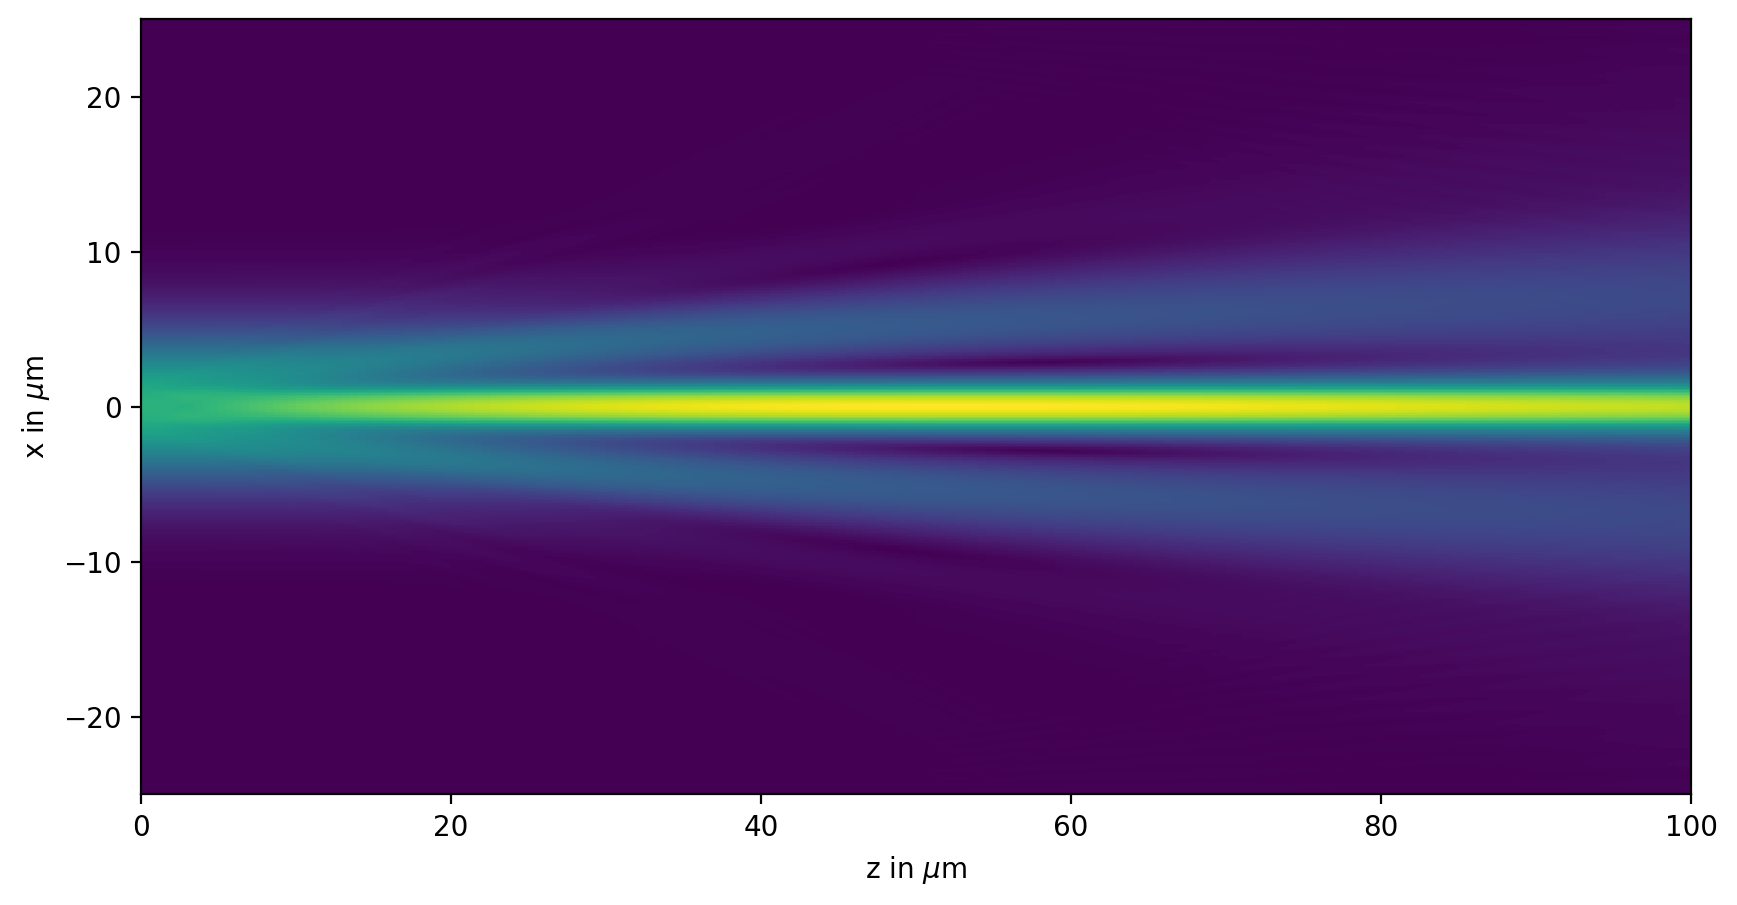
\includegraphics[width=.9\textwidth]{figures/index.png}
        \caption{Propagation of a Gaussian beam with $w=\SI{5}{\micro\meter}$, $\Delta z=\SI{0.5}{\micro\meter}$, $\lambda=\SI{1}{\micro\meter}$,  $\Delta x=\SI{0.5}{\micro\meter}$ , $x_b=\SI{2}{\micro\meter}$,
         $n_\text{cladding}=1.46$, $n_\text{core}=1.45$, $\bar k = k_0 \cdot 1.455$.}
        \label{fig:simres}
    \end{figure}
    We observe that only the central part of the Gaussian beam is guided since
    the waveguide's width is smaller than the beam's. Hence, the non-central part spreads out.
        \begin{figure}[H]
        \centering
        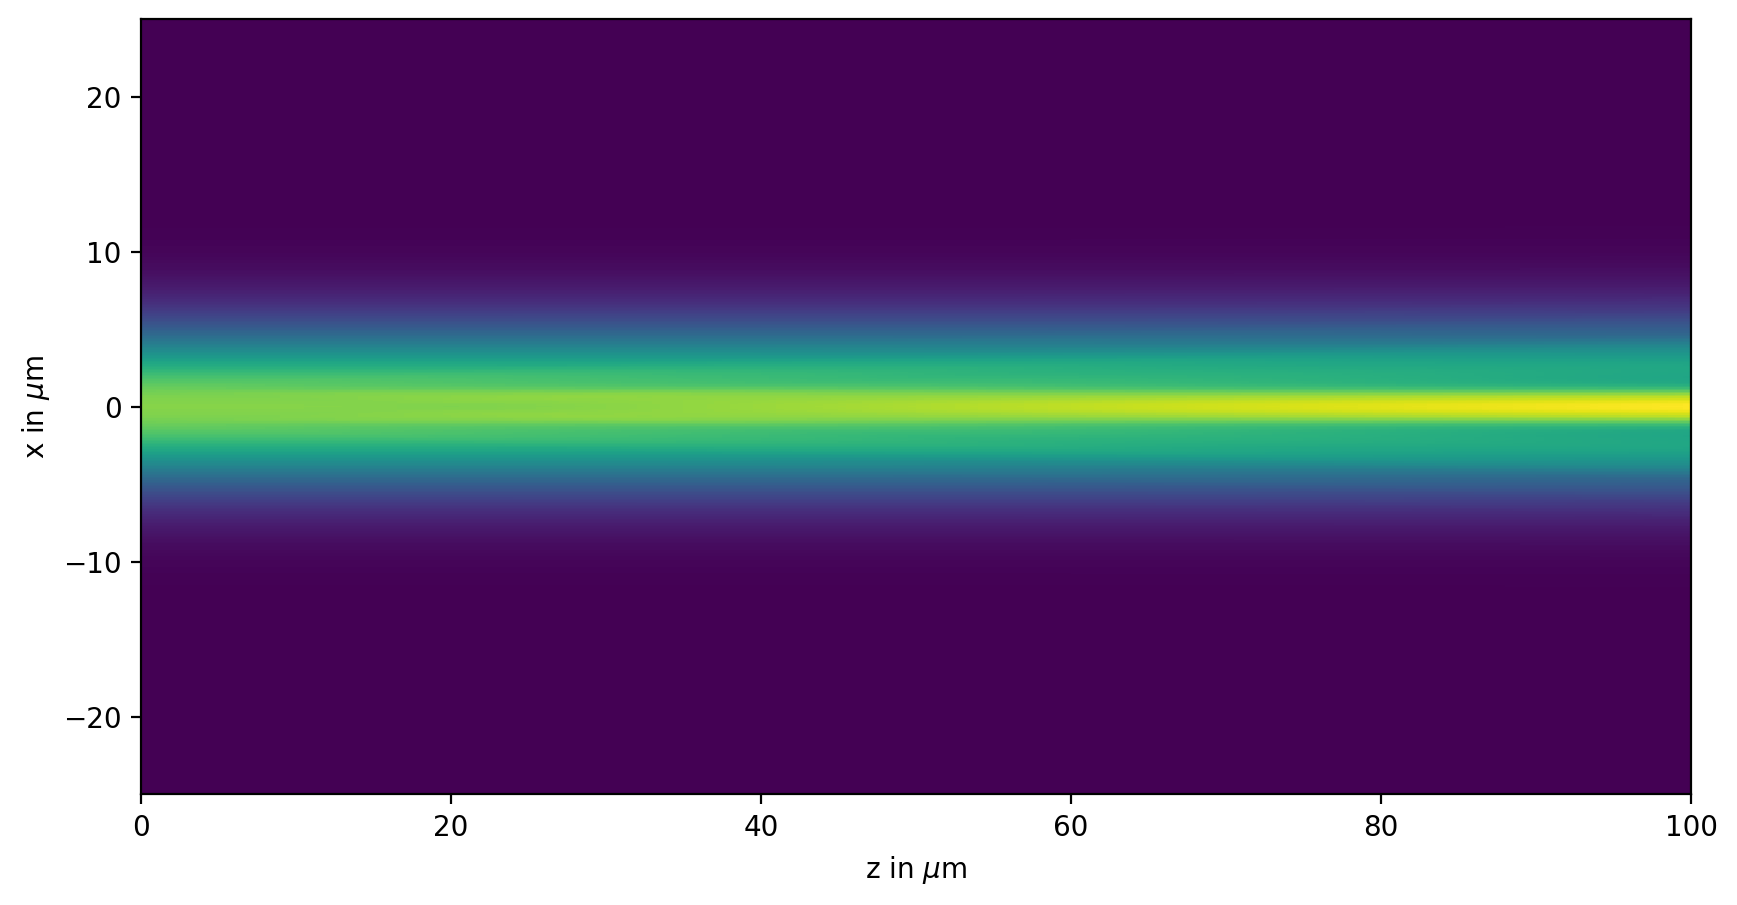
\includegraphics[width=.9\textwidth]{figures/index_kbar=3.png}
        \caption{Propagation of a Gaussian beam with the same parameters
        as in \autoref{fig:simres}, but $\bar k = k_0 \cdot 3$.}
        \label{fig:simres2}
    \end{figure}
    In \autoref{fig:simres2} we can observe the effect when $\bar k$ is chosen too large. The approximation of a slowly varying amplitude is violated and the two figures are not identical.
    The figure indicates that the beam would be better guided.
    One effect due to the perfectly conducting boundaries can be seen in 
    \autoref{fig:simrespec}.
    \begin{figure}[H]
        \centering
        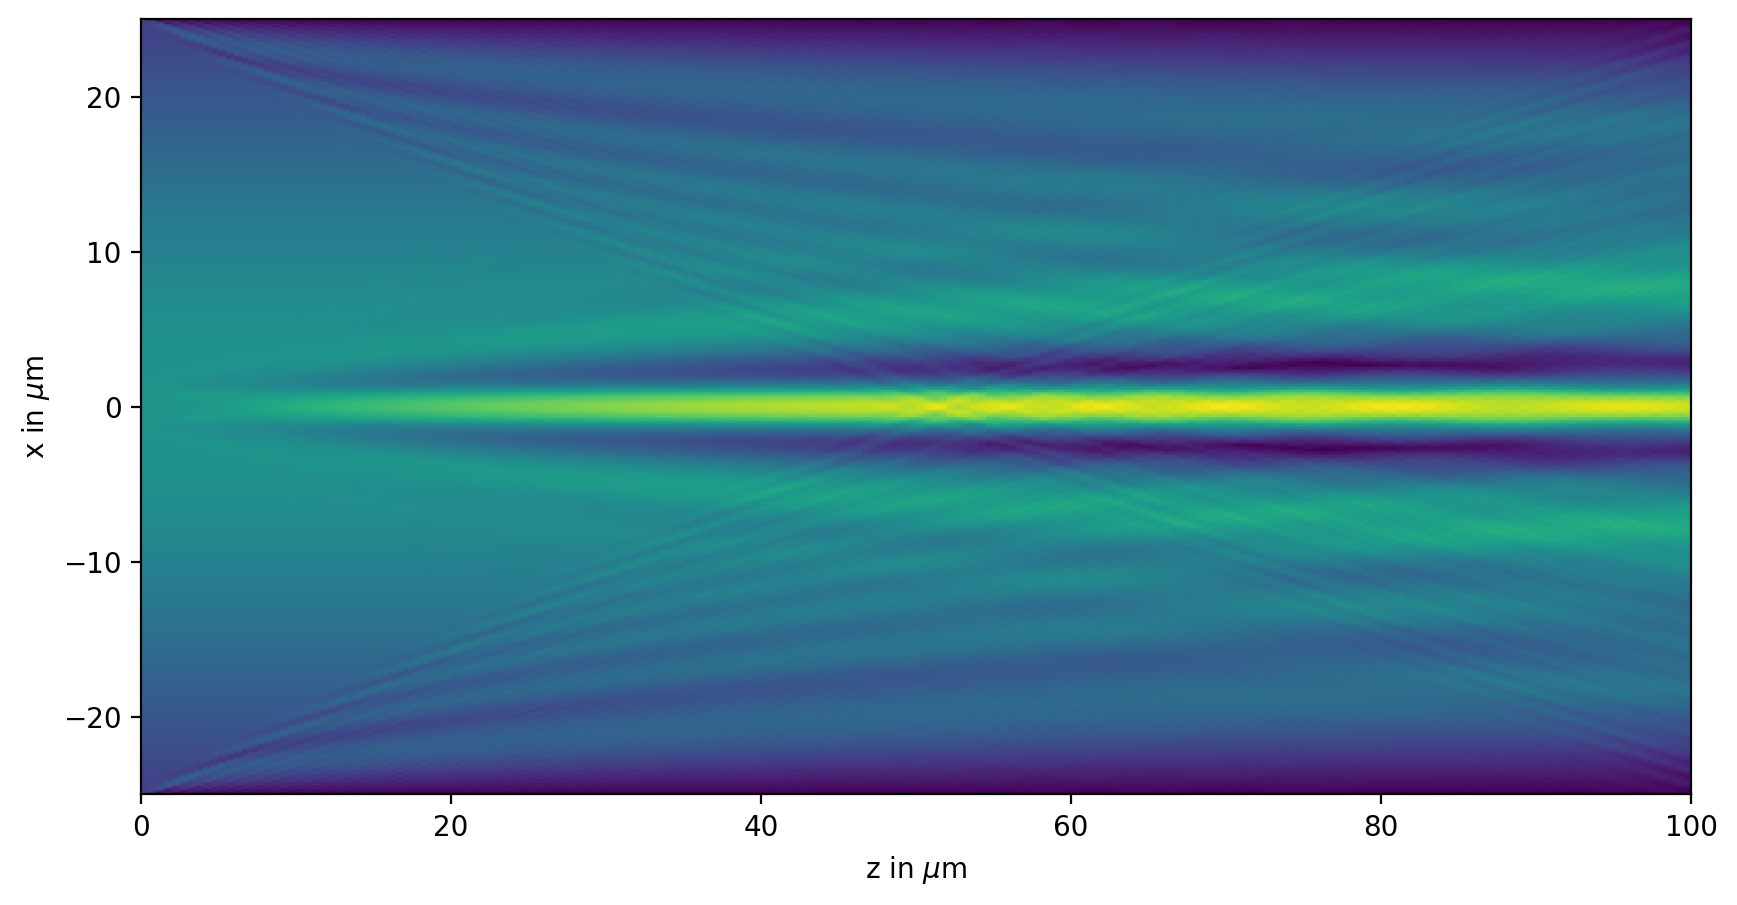
\includegraphics[width=.9\textwidth]{figures/index_w=25.png}
        \caption{Propagation of a Gaussian beam with the same parameters
        as in \autoref{fig:simres} but $w=\SI{25}{\micro\meter}$.}
        \label{fig:simrespec}
    \end{figure}
    Some waves are reflected at the top and the bottom. Therefore one needs to choose a larger simulation grid or more suitable boundary conditions.
    
    \subsection{Computational Performance}
        Furthermore we provide some data for the computational performance.
        Our setup for all measurements was Python 3.8.2, SciPy 1.3.2, NumPy 1.17.3 and a Intel(R) Core(TM) i7-7600U CPU @ 2.80GHz. The datatype for the performance critical part was single float.
        For the parameters of \autoref{fig:simres} the elapsed time of the
        LU method was \SI{0.012\pm0.001}{\second}. 
        Instead of doing the factorization, we could also solve the
        system of equations in every step via \pythoninline{spsolve}.
        For this the elapsed time was \SI{0.044\pm 0.005}{\second}. So doing the factorization already improves the performance by a factor of 4.
        The slowest approach is the explicit inversion (once before the \pythoninline{for}-loop) of \pythoninline{Ml}. This approach takes \SI{0.81\pm0.01}{\second}, being a factor of roughly 70 slower than the factorization.
        
    \subsection{Convergence Rate}
        We can vary the step sizes both $\Delta z$ and $\Delta x$ to check the convergence rate. By theory it is quadratically convergent for both lateral
        and traversal step size.
        First we can calculate a reference field with high resolution in $x$.
        Then we simulate another field with a lower $x$ resolution.
        To compare the high resolution field with the low resolution field,
        we need to downscale the high resolution field to be the same size 
        as the smaller one.
        After the downscaling we can calculate the mean 
        error of the fields via:
        \begin{equation}
            \text{error}_x = \frac{1}{N_x} \sum_{i} \left| |A_i^n| - |A_i^\text{ref}| \right| 
        \end{equation}
        where $A_i^\text{ref}$ is the high resolution reference field. Because the field values in general are complex, we use the absolute values.
        In \autoref{fig:simfitx} we see the error plotted over the different step sizes $\Delta x$. The orange curve indicates a fitted function $a \cdot ( \Delta x)^b$ with $a=\SI{3.36\pm0.02e-5}{}$ and $b= 2.09 \pm 0.01$. $b$ is the rate of convergence. Since $b$ is larger than $2$ we observe a convergence
        which is slightly higher than expected.
        \begin{figure}[H]
            \centering
            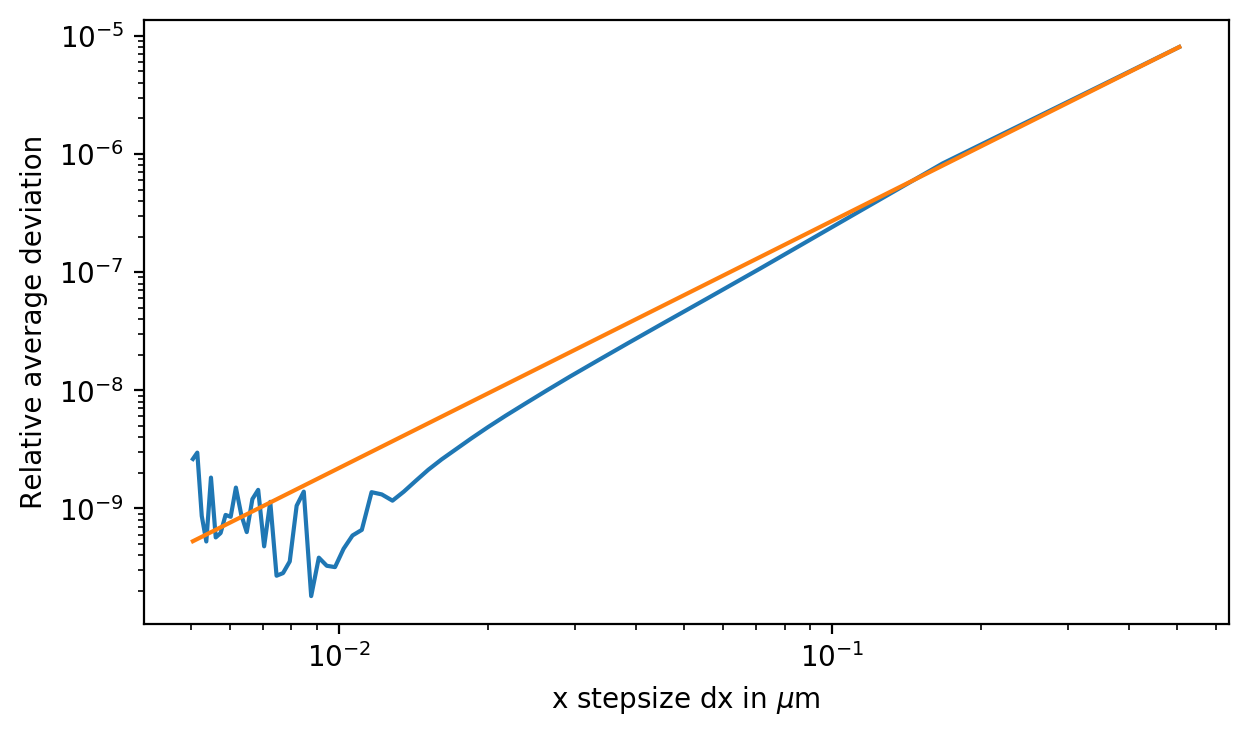
\includegraphics[width=.8\textwidth]{figures/fit_x.png}
            \caption{Convergence behaviour with different $x$ sampling.
            Same set of parameters as in \autoref{fig:simres}.}
            \label{fig:simfitx}
        \end{figure}
        For the error with different $\Delta z$ we do not need to scale the reference field because we can only evaluate the field at the final $z$ position. \autoref{fig:simfitz} shows the convergence behaviour for different
        $z$ sampling. The fitted parameters of the orange curve are $a=\SI{5.08\pm0.06e-5}{}$ and $b = 0.96 \pm 0.02$. For $z$ the convergence is therefore one order lower than expected. For the difference we do not have a reasonable explanation.
        \begin{figure}[H]
            \centering
            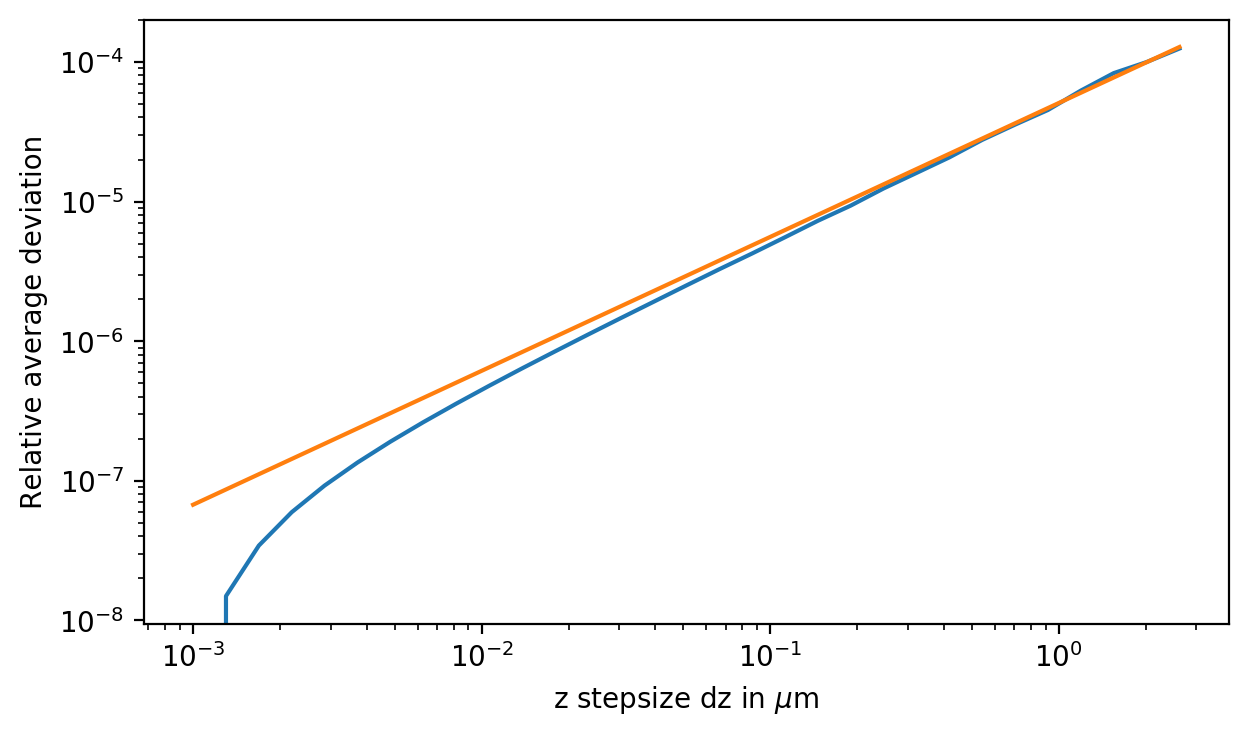
\includegraphics[width=.8\textwidth]{figures/fit_z.png}
            \caption{Convergence behaviour with different $z$ sampling.
            Same set of parameters as in \autoref{fig:simres}.}
            \label{fig:simfitz}
        \end{figure}
        
        
\section{Conclusion}
    In this report we presented the physical background of the beam propagation. Following we showed details of the numerical implementation
    and the discretization in propagation direction $z$ and traversal coordinate $x$. 
    Additionally we included considerations on computation efficiency, regarding the solving of the principal equation.
    At the end we provided some insights into the convergence behaviour of the Crank-Nicolson scheme. Despite the method being a second order method we did not achieve the same convergence rate for $\Delta z$. For $\Delta x$  we were able to confirm the convergence order.
    
\newpage
%to print all entries
\nocite{*}
\printbibliography


\end{document}